%This is the Preface
%%=========================================
\addcontentsline{toc}{section}{Abstract}
\section*{Abstract}

Internet of Things (IoT) applications very often involve the use of sensors. Motion sensing can be used in a vast amount of applications and are therefore very interesting in high volume IoT products. Replacing a battery in such an application is often undesirable, and may in some cases be close to impossible. It is therefore essential for such applications to have sensors that consumes as little power as possible. 

This project thesis presents a thorough analysis of five commercially available micro electromechanical (MEMS) 3-axis accelerometers. The analysis focuses primarily on finding the sensor that gives the best trade-off between functionality and power consumption. 

This thesis further explores different techniques to acquire data from the sensor with the lowest possible power consumption. A custom development board was made specifically for this purpose.

The project is carried out as feasibility analysis for Disruptive Technologies AS in conjunction with the Norwegian University of Science and Technology (NTNU).

[Future work might be to look at the possibility of bonding together one of the MEMS products with a proprietary IC.]


\begin{center}
Trondheim, 2015-12-16\\[1pc]
\begin{figure}[h]
\centering
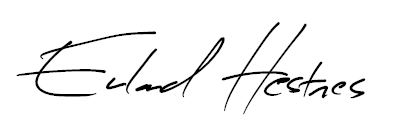
\includegraphics[scale=0.5]{fig/underskrift.png}
\label{fig:underskrift}
\end{figure}
Erlend Hestnes
\end{center}